\chapter{Specifikacija programske potpore}

\section{Funkcionalni zahtjevi}

\noindent \textbf{Dionici:} 
\begin{enumerate}
	\item Organizator kampa (naručitelj)
	\item Sudionici kampa
	\item Animatori
	\item Administrator
	\item Razvojni tim\\
\end{enumerate}

\noindent \textbf{Aktori i njihovi funkcionalni zahtjevi: } 

\begin{enumerate}
	\item \underbar{Neregistrirani/neprijavljeni korisnik (inicijator) može:} 
	\begin{enumerate}
		\item vidjeti osnovne informacije o kampu
		\item vidjeti vrijeme održavanja, trajanja i popis aktivnosti
		\item prijaviti se na prijavu za sudjelovanje u kampu ili na prijavu za animatora gdje upisuju svoje puno ime, e-mail adresu, broj telefona, datum i godinu rođenja i motivacijsko pismo
		\item sudionici koji imaju manje od 18 godina moraju unijeti i broj telefona odgovorne osobe
		\item biti obaviješten o tome je li njegova prijava prihvaćena putem e-maila \\
	\end{enumerate} 
	\item \underbar{Sudionik (inicijator) može: }
	\newline Nakon prijave u sustav prije početka kampa:
	\begin{enumerate}
		\item prilikom registracije upisati lozinku za dobiveno korisničko ime
		\item vidjeti odbrojavanje do početka kampa
		\item kontaktirati organizatora
	\end{enumerate}
	Nakon početka kampa:
	\begin{enumerate}
		\item vidjeti stranicu s rasporedom ili agendom
		\item vidjeti popis članova svoje grupe i animatore i njihove kontakt podatke
		\item vidjeti popis aktivnosti na kojima su sudjelovali i ocijeniti aktivnost (1-10) i ostaviti kratak opis dojma
	\end{enumerate}
	Nakon završetka kampa:
	\begin{enumerate}
		\item ocijeniti cjelokupno iskustvo i ostaviti vlastiti dojam\\
	\end{enumerate}
	
	\item \underbar{Animator (inicijator) može: }
	\newline Nakon prijave u sustav prije početka kampa:
	\begin{enumerate}
		\item prilikom registracije upisati lozinku za dobiveno korisničko ime
		\item vidjeti odbrojavanje do početka kampa
		\item kontaktirati organizatora
	\end{enumerate}
	Nakon početka kampa:
	\begin{enumerate}
		\item vidjeti stranicu s rasporedom ili agendom
		\item vidjeti popis svih grupa, njihovih članova i popis drugih animatora te njihove kontakt podatke
		\item vidjeti popis aktivnosti na kojima su animirali i ocijeniti aktivnost (1-10) i ostaviti kratak opis dojma
	\end{enumerate}	
	Nakon završetka kampa:
	\begin{enumerate}
		\item ocijeniti cjelokupno iskustvo i ostaviti vlastiti dojam\\
	\end{enumerate}
	
	\item \underbar{Organizator (inicijator) može: }
	\begin{enumerate}
		\item zadati početne informacije o kampu (vrijeme održavanja, trajanje, aktivnosti)
		\item jednostavno definirati aktivnost (ime, kratki opis, trajanje)
		\item omogućiti prijave za kamp i odrediti vrijeme trajanja prijavi
		\item vidjeti popis prijava te ih odbiti ili prihvatiti
		\item nakon završetka odabira prijava određivati broj grupa u koje će sudionici biti raspoređeni	
		\item popuniti raspored s aktivnostima uz određene uvjete i aktivnostima pridružiti grupe
		\item vidjeti popis svih povratnih ocjena po aktivnostima
		\item pretraživati povratne ocjene po atributima korisnik, grupa i/ili aktivnost\\
	\end{enumerate}
	
	\item \underbar{Administrator (inicijator) može: }
	\begin{enumerate}
		\item vidjeti popis svih registriranih korisnika
		\item brisati i dodavati korisnike i davati im ovlaštenja i mijenjati im razinu pristupa (organizator, sudionik, animator)
		\item slučajnim odabirom rasporediti sudionike u grupe
		\item premještati sudionika iz grupe u grupu
		\item nakon prihvaćene prijave stvoriti korisnički račun i poslati e-mail korisniku	
		\item ako je odbijena prijava obavijestiti korisnika e-mailom
		\item micati dojmove čije riječi nisu sukladne pravilima korištenja stranice\\
	\end{enumerate}
	
	\item \underbar{Baza podataka (sudionik): }
	
	\begin{enumerate}
		\item pohranjuje sve podatke o korisnicima i njihovim ovlastima
		\item pohranjuje sve podatke o aktivnostima i grupama
		\item pohranjuje krajnje dojmove
	\end{enumerate}
	
	
\end{enumerate}



\newpage
\subsection{Obrasci uporabe}
\subsubsection{Opis obrazaca uporabe}

\noindent \underbar{\textbf{UC1 - Organizacija kampa}}
\begin{itemize}
	\item \textbf{Glavni sudionik:} Organizator
	\item \textbf{Cilj:} Postaviti osnovne informacije o kampu
	\item \textbf{Sudionici:} Baza podataka
	\item \textbf{Preduvjet:} Organizator mora biti evidentiran u bazi
	\item \textbf{Opis osnovnog tijeka:} 
	\begin{enumerate}	
		\item Organizator se prijavljuje kroz web aplikaciju
		\item Organizator kroz sučelje za izradu kampa unosi podatke
		\item Organizator odabire gumb kreacije kampa\\
	\end{enumerate}
	
\end{itemize}

\noindent \underline{\textbf{UC2 - Kreiranje aktivnosti}}

\begin{itemize}
	\item \textbf{Glavni sudionik:} Organizator
	\item \textbf{Cilj:} Napraviti novu aktivnost
	\item \textbf{Sudionici:} Baza podataka
	\item \textbf{Preduvjet:} -
	\item \textbf{Opis osnovnog tijeka:} 
	\begin{enumerate}	
		\item Organizator odabire sučelje za kreaciju nove aktivnosti
		\item Organizator odabire detalje nove aktivnosti
		\item Detalji nove aktivnosti se prikazuju organizatoru koji ih može potvrditi te tako završiti proces kreacije
	\end{enumerate}
	
\end{itemize}

\noindent \underline{\textbf{UC3 - Zadavanje trajanja prijave}}
\begin{itemize}
	\item \textbf{Glavni sudionik:} Organizator
	\item \textbf{Cilj:} Odrediti vrijeme prijave za sudionike i animatore
	\item \textbf{Sudionici:} Baza podataka
	\item \textbf{Preduvjet:} Organizator mora biti evidentiran u bazi
	\item \textbf{Opis osnovnog tijeka:} 
	\begin{enumerate}	
		\item Organizator odabire sučelje za određivanje trajanja prijave
		\item Organizator odabire vrijeme trajanja prijave i za koga je prijava namijenjena
		\item Otvara se mogućnost prijave u zadanom terminu\\
	\end{enumerate}
	
\end{itemize}

\noindent \underline{\textbf{UC4 - Prijava za sudjelovanje}}
\begin{itemize}
	\item \textbf{Glavni sudionik:} Potencijalni sudionik (neregistrirani korisnik)
	\item \textbf{Cilj:} Prijava za sudjelovanje na kampu
	\item \textbf{Sudionici:} Baza podataka
	\item \textbf{Preduvjet:} -
	\item \textbf{Opis osnovnog tijeka:} 
	\begin{enumerate}	
		\item Korisnik odabire sučelje za prijavu za sudionika na kamp
		\item Korisnik upisuje tražene podatke
		\item Prijava se prikazuje organizatoru koji dalje može prihvatiti ili odbiti prijavu\\
	\end{enumerate}
\end{itemize}


\noindent \underline{\textbf{UC5 - Potvrda prijave sudionika}}
\begin{itemize}
	\item \textbf{Glavni sudionik:} Organizator
	\item \textbf{Cilj:} Potvrditi prijavu sudionika
	\item \textbf{Sudionici:} Baza podataka
	\item \textbf{Preduvjet:} Sudionik mora poslati prijavu 
	\item \textbf{Opis osnovnog tijeka:} 
	\begin{enumerate}	
		\item Organizator prihvaća prijavu
		\item Organizator šalje prihvaćenom sudioniku link za registraciju na e-mail naveden u prijavi\\
	\end{enumerate}
	
\end{itemize}


\noindent \underline{\textbf{UC6 - Odbijanje prijave sudionika}}
\begin{itemize}
	\item \textbf{Glavni sudionik:} Organizator
	\item \textbf{Cilj:} Odbiti prijavu sudionika
	\item \textbf{Sudionici:} Baza podataka
	\item \textbf{Preduvjet:} Sudionik mora poslati prijavu
	\item \textbf{Opis osnovnog tijeka:} 
	\begin{enumerate}	
		\item Organizator odbija prijavu
		\item Organizator šalje sudioniku obavijest o odbijanju na e-mail naveden u prijavi\\
	\end{enumerate}
	
\end{itemize}


\noindent \underline{\textbf{UC7 - Prijava za animatore}}
\begin{itemize}
	\item \textbf{Glavni sudionik:} Potencijalni animator (neregistrirani korisnik)
	\item \textbf{Cilj:} Prijava za posao animatora na kampu
	\item \textbf{Sudionici:} Baza podataka
	\item \textbf{Preduvjet:} -
	\item \textbf{Opis osnovnog tijeka:} 
	\begin{enumerate}	
		\item Korisnik odabire sučelje za prijavu za animatora na kamp
		\item Korisnik upisuje tražene podatke
		\item Prijava se prikazuje organizatoru koji dalje može prihvatiti ili odbiti prijavu\\
	\end{enumerate}
	
\end{itemize}

\noindent \underline{\textbf{UC8 - Registracija sudionika}}
\begin{itemize}
	\item \textbf{Glavni sudionik:} Sudionik
	\item \textbf{Cilj:} Registracija sudionika
	\item \textbf{Sudionici:} Baza podataka
	\item \textbf{Preduvjet:} Prihvaćena prijava od strane organizatora
	\item \textbf{Opis osnovnog tijeka:} 
	\begin{enumerate}	
		\item Korisnik dobiva mail sa podatcima za registraciju
		\item Korisnik upisuje proizvoljnu lozinku na sučelju za registraciju
		\item Registracija se evidentira u bazi podataka\\
	\end{enumerate}
	
\end{itemize}


\noindent \underline{\textbf{UC9 - Razmještaj sudionika po grupama}}
\begin{itemize}
	\item \textbf{Glavni sudionik:} Organizator
	\item \textbf{Cilj:} Razmjestiti sudionike po grupama
	\item \textbf{Sudionici:} Baza podataka
	\item \textbf{Preduvjet:} Organizator je završio odabir prijava
	\item \textbf{Opis osnovnog tijeka:} 
	\begin{enumerate}	
		\item Organizator određuje broj grupa za sudionike
		\item Grupa svakog sudionika se evidentira u bazi podataka\\
	\end{enumerate}
	
\end{itemize}

\noindent \underline{\textbf{UC10 - Zahtjev za premještanje}}
\begin{itemize}
	\item \textbf{Glavni sudionik:} Sudionik
	\item \textbf{Cilj:} Zatražiti premještaj u drugu grupu
	\item \textbf{Sudionici:} Baza podataka
	\item \textbf{Preduvjet:} Sudionici su raspoređeni po grupama
	\item \textbf{Opis osnovnog tijeka:} 
	\begin{enumerate}	
		\item Sudionik odabire opciju zahtjeva za premještaj 
		\item Sudioniku se izlistaju ostale grupe
		\item Sudionik odabire željenu grupu\\
	\end{enumerate}
	
\end{itemize}


\noindent \underline{\textbf{UC11 - Premještaj pojedinog sudionika u drugu grupu}}
\begin{itemize}
	\item \textbf{Glavni sudionik:} Organizator
	\item \textbf{Cilj:} Premjestiti sudionika u drugu grupu
	\item \textbf{Sudionici:} Baza podataka
	\item \textbf{Preduvjet:} Zahtjev za premještaj
	\item \textbf{Opis osnovnog tijeka:} 
	\begin{enumerate}	
		\item Organizator zaprima zahtjev za premještaj sudionika u drugu grupu
		\item Premještaj se evidentira u bazi podataka\\
	\end{enumerate}
	
\end{itemize}


\noindent \underline{\textbf{UC12 - Punjenje rasporeda i provjera aktivnosti}}
\begin{itemize}
	\item \textbf{Glavni sudionik:} Organizator
	\item \textbf{Cilj:} Popuniti raspored s aktivnostima i provjeriti kršenje uvjeta aktivnosti
	\item \textbf{Sudionici:} Baza podataka
	\item \textbf{Preduvjet:} Formirane su grupe
	\item \textbf{Opis osnovnog tijeka:} 
	\begin{enumerate}	
		\item Aktivnost se neće preklapati s aktivnošću istog tipa
		\item Pridružen je minimalno jedan animator
		\item Pridružen je odgovarajući broj grupa
		\item Nijedna od pridruženih grupa neće imati konflikte s drugim aktivnostima koje su već
		navedene
		\item  Nijedna od pridruženih grupa nije već pridružena jednakoj aktivnosti
		\item Pridruženi animatori neće imati konflikte s drugim aktivnostima na koje su pridruženi\\
	\end{enumerate}
	
\end{itemize}



\noindent \underline{\textbf{UC13 - Ocjenjivanje aktivnosti}}
\begin{itemize}
	\item \textbf{Glavni sudionik:} Sudionici i animatori
	\item \textbf{Cilj:} Dati povratnu ocjenu za aktivnosti
	\item \textbf{Sudionici:} Baza podataka
	\item \textbf{Preduvjet:} Aktivnost je završila
	\item \textbf{Opis osnovnog tijeka:} 
	\begin{enumerate}	
		\item Sudionici i organizatori ocjenjuju aktivnost
		\item Ocjene se evidentiraju u bazi podataka
		\item Organizator može pretraživati ocjene\\
	\end{enumerate}
\end{itemize}


\noindent \underline{\textbf{UC14 - Ocjenjivanje cjelokupnog iskustva}}
\begin{itemize}
	\item \textbf{Glavni sudionik:} Sudionici i animatori
	\item \textbf{Cilj:} Dati povratnu ocjenu za cjelokupno iskustvo
	\item \textbf{Sudionici:} Baza podataka
	\item \textbf{Preduvjet:} Kamp je završio
	\item \textbf{Opis osnovnog tijeka:} 
	\begin{enumerate}	
		\item Sudionici i organizatori ocjenjuju cjelokupno iskustvo
		\item Ocjene se evidentiraju u bazi podataka
		\item Organizator može pretraživati ocjene\\
	\end{enumerate}
\end{itemize}

\subsubsection{Dijagrami obrazaca uporabe}

\begin{figure}[H]
	\centering
	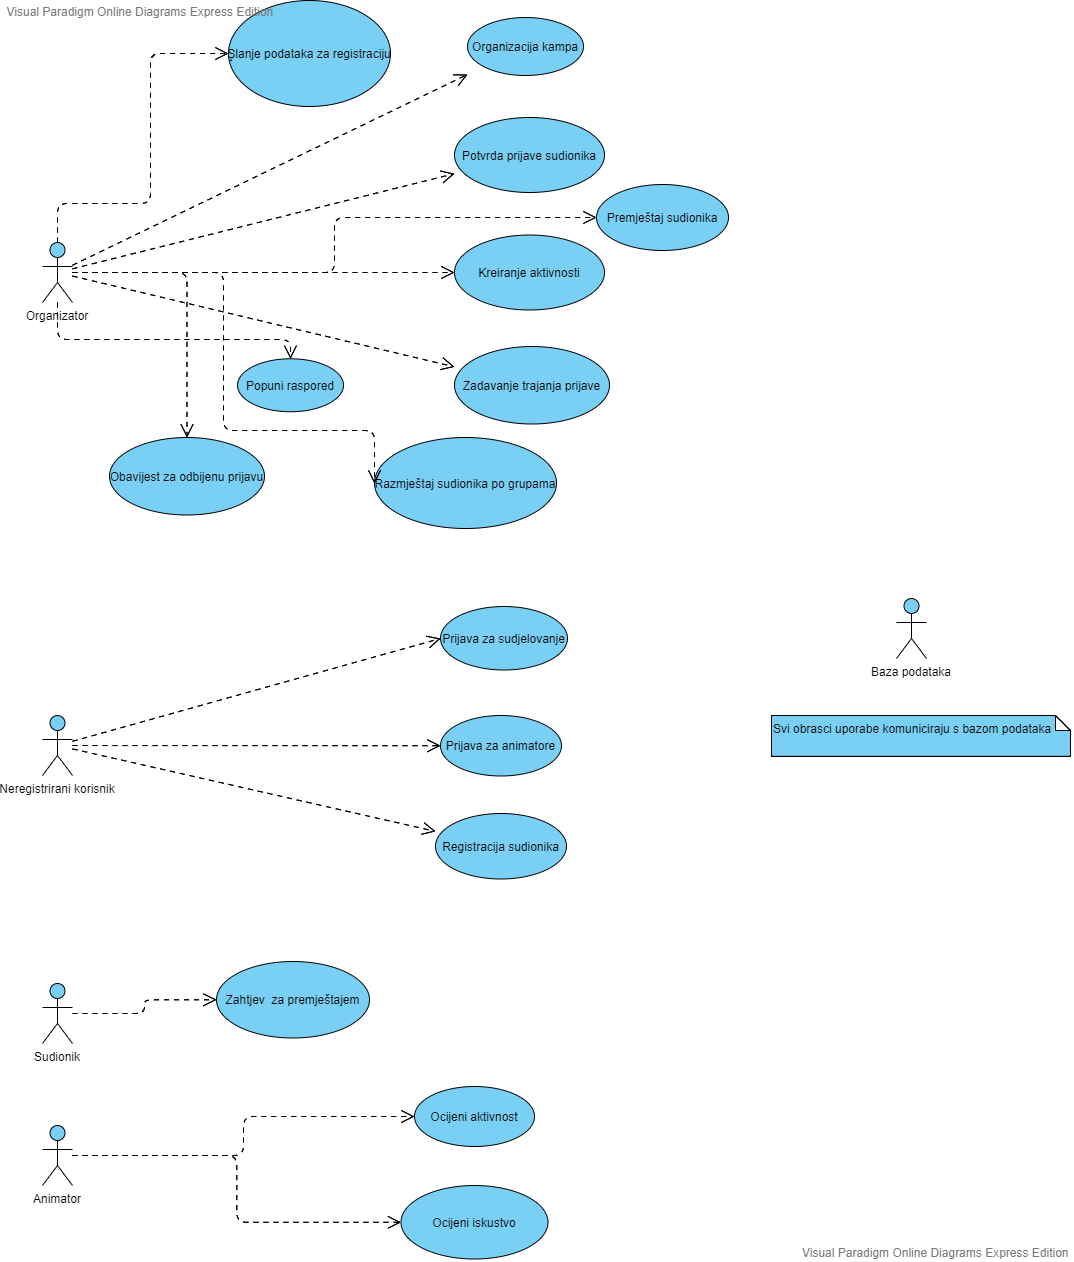
\includegraphics[scale=0.45]{dijagrami/dijagramObrazacaUporabe.PNG}
	\caption{Dijagram obrazaca uporabe}
\end{figure}
\newpage

\subsection{Sekvencijski dijagrami}\label{sec:sekvencijski-dijagrami}
\textbf{Obrazac upotrebe UC1 - Organizacija kampa}\\
\begin{figure}[H]
	\centering
	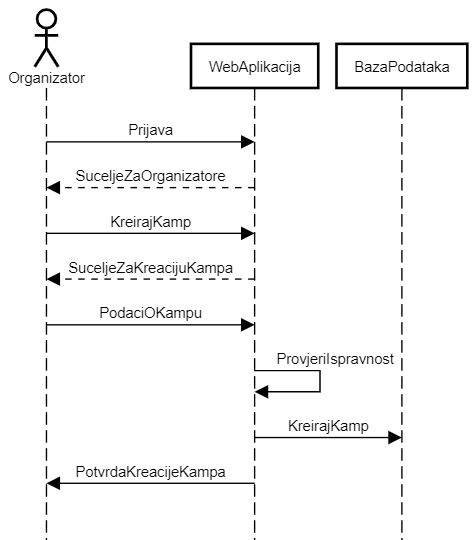
\includegraphics[scale=0.6]{dijagrami/UC1.PNG}
	\caption{Sekvencijski dijagram za UC1}
	\label{fig: uc1 sekv}
\end{figure}

%===========================================================
\newpage
\textbf{Obrazac upotrebe UC2 - Kreiranje aktivnosti}
\begin{figure}[H]
	\centering
	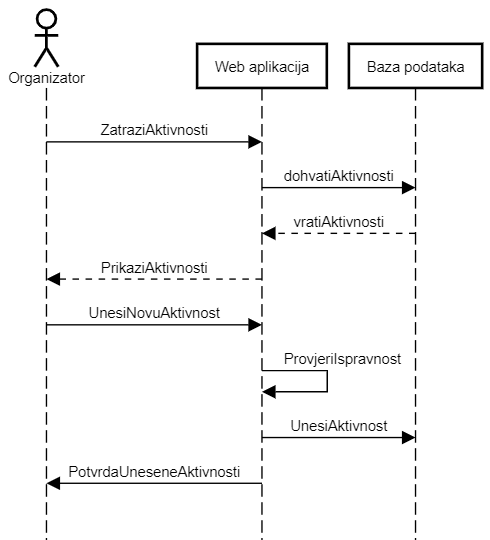
\includegraphics[scale=0.6]{dijagrami/UC2.PNG}
	\caption{Sekvencijski dijagram za UC2}
	\label{fig: uc2 sekv}
	\label{fig: uc2 sekv}
\end{figure}

%===========================================================
\newpage
\textbf{Obrazac upotrebe UC3 - Zadavanje trajanja prijave}
\begin{figure}[H]
	\centering
	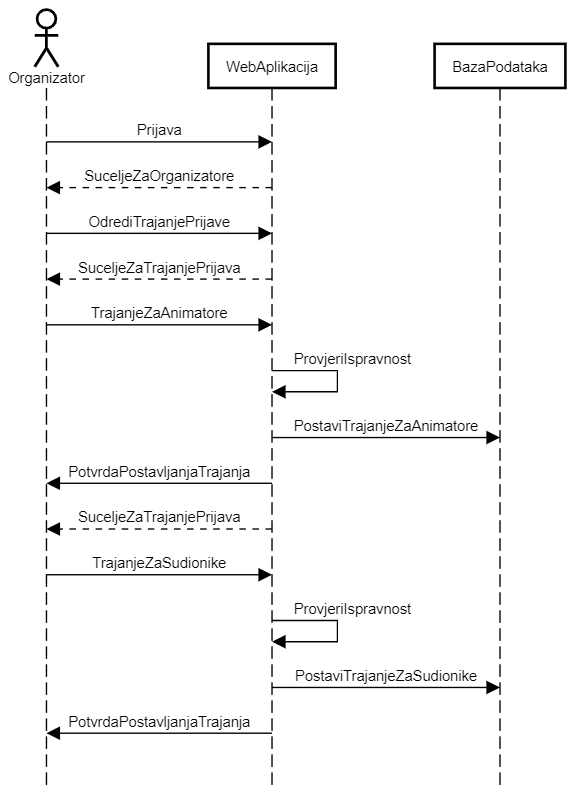
\includegraphics[scale=0.6]{dijagrami/UC3.PNG}
	\caption{Sekvencijski dijagram za UC3}
	\label{fig: uc3 sekv}
\end{figure}


%===========================================================
\newpage
\textbf{Obrazac upotrebe UC4 - Prijava za sudjelovanje}
\begin{figure}[H]
	\centering
	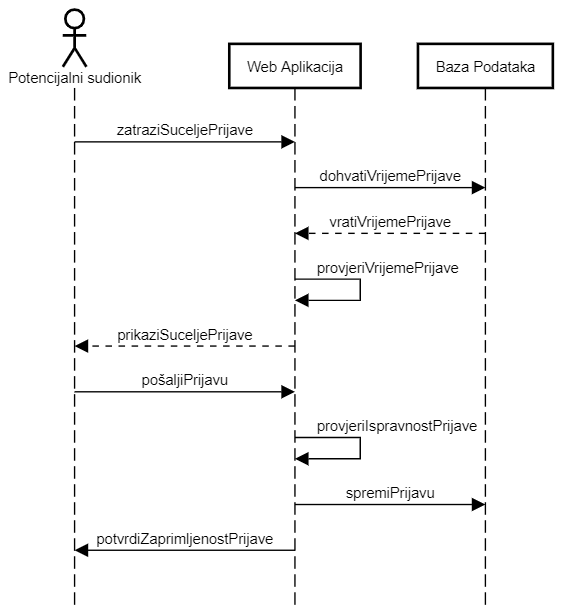
\includegraphics[scale=0.6]{dijagrami/UC4.PNG}
	\caption{Sekvencijski dijagram za UC4}
	\label{fig: uc4 sekv}
\end{figure}


\newpage
\section{Ostali zahtjevi}
\begin{itemize}
	\item sustav treba biti implementiran kao web aplikacija koristeći objektno-orijentirane jezike
	\item korisničko sučelje i sustav moraju podržavati hrvatsku abecedu (dijakritičke znakove) pri unosu i prikazu tekstualnog sadržaja
	\item nadogradnja sustava ne smije narušavati postojeće funkcionalnosti sustava
	\item neispravno korištenje korisničkog sučelja ne smije narušiti funkcionalnost i rad sustava
	\item sustav treba biti jednostavan za korištenje, korisnici se moraju znati koristiti sučeljem bez opširnih uputa
	\item sustav treba omogućiti rad više korisnika u stvarnom vremenu
	\item izvršavanje dijela programa u kojem se pristupa bazi podataka ne smije trajati duže od nekoliko sekundi
	\item pristup sustavu mora biti omogućen iz javne mreže
\end{itemize}